% LaTeX format of Model Validation for Baruch 2017 MTH9845 Risk Management class
%
% Created by: Hongchao Pan & Yu Sun
% Version 1.0
% Date: 04/25/2017
% Contact Info: hpan.baruch@gmail.com & yusun.baruch@gmail.com
%
% Just compile this main file

\documentclass[12pt,a4paper]{report}
\usepackage{amsmath} %for greeks
\usepackage[pdftex]{graphicx} %for embedding images
\usepackage{url} %for proper url entries
\usepackage[bookmarks, colorlinks=false, pdfborder={0 0 0}, pdftitle={MTH9845 Model Validation}, pdfauthor={Hongchao Pan and Yu Sun}, pdfsubject={<subject here>}, pdfkeywords={<keywords here>}]{hyperref} %for creating links in the pdf version and other additional pdf attributes, no effect on the printed document
%\usepackage[final]{pdfpages} %for embedding another pdf, remove if not required

\newtheorem{prop}{Proposition}

\begin{document}
\renewcommand\bibname{References} %Renames "Bibliography" to "References" on ref page

%include other pages
\begin{titlepage}

% Add Baruch Logo

\includegraphics[width=0.5\textwidth]{./MFE-Logo}\\[0.2in]

\begin{center}

\textup{\Large {\bf MTH9845 Risk Management} \\ [0.2in] Model Validation Report}\\[0.2in] \textit{with}\\[0.2in]

% Title
\Large \textbf {{Vanna-Volga Pricing Model }\\ for FX options} \\ [1in]

%       \small \emph{Submitted in partial fulfillment of\\
%        the requirements for the award of the degree of}
%        \vspace{.2in}

%       {\bf Bachelor of Technology \\in\\ Computer Science and Engineering}\\[0.5in]

% Submitted by
\normalsize Submitted by \\
\begin{table}[h]
\centering
\begin{tabular}{cc}\hline \\
Names of Studens & Emails \\ \\ \hline
\\
Hongchao Pan & hpan.baruch@gmail.com \\[0.1in]
Yu Sun & yusun.baruch@gmail.com \\ \\ \hline 
\end{tabular}
\end{table}

\vspace{.1in}
%Under the guidance of\\
%{\textbf{<Guide's name here>}}\\[0.2in]

\vfill

% Bottom of the page
\Large{Master of Financial Engineering}\\
\normalsize
\textsc{Baruch College, CUNY}\\
New York , NY, USA -- 10010 \\
\vspace{0.2cm}
Spring Semester 2017

\end{center}

\end{titlepage}

%\newpage
\thispagestyle{empty}

\begin{center}

\huge{Department of Computer Science and Engineering}\\[0.5cm]
\normalsize
\textsc{National Institute of Technology Calicut}\\[2.0cm]

\emph{\LARGE Certificate}\\[2.5cm]
\end{center}
\normalsize This is to certify that this is a bonafide record of the project presented by the students whose names are given below during <Monsoon/Winter and Year here> in partial fulfilment of the requirements of the degree of Bachelor of Technology in Computer Science and Engineering.\\[1.0cm]

\begin{table}[h]
\centering
\begin{tabular}{lr}
Roll No & Names of Students \\ \\ \hline
\\
<Roll no here> & <Name here> \\ 
<Roll no here> & <Name here> \\
<Roll no here> & <Name here> \\
\end{tabular}
\end{table}

\vfill


% Bottom of the page
\begin{flushright}
<Guide name here>\\
(Project Guide)\\[1.5cm]
<Coordinator name here>\\
(Course Coordinator)\\
\end{flushright}

\begin{flushleft}
Date:
\end{flushleft}
 % Not need this for our model validation report
%\vspace{2in}
\begin{abstract}

<Abstract here>

\end{abstract} 
  % Not need this for our model validation report

\pagenumbering{roman} %numbering before main content starts
\tableofcontents
\listoffigures

\newpage
\pagenumbering{arabic} %reset numbering to normal for the main content

\chapter{Executive Summary}
This paper examines the validity of Vanna-Volga Pricing method, a technique for pricing options in Foreign Exchange (FX) markets. \newline
The Foreign Exchange option's market is the largest and most liquid market of options in the world. Numerous shares of options, ranging from simple vanilla options to exotics options, are traded everyday. Thus, it is imperative for any pricing model to provide a rapid and accurate mark-to-market price calculation.\newline
The most straightforward model would be Black-Scholes model, which could derive analytical prices based on several unrealistic assumptions. It is clearly wrong to assume that the interest rate and FX-spot volatility would remain constant throughout the the maturity of the option. These two factors would be assumed to follow stochastic processes in more realistic models, such as Heston model and SABR volatility model. These models are accurate and rigorous, while normally they are computationally demanding, complex to implement and need delicate calibration. \newline
As an alternative approach, the Vanna-Volga method provide price adjustment for smile impact. It has easy implementation, efficient computation and simple or no calibration. It takes a small amount of market quotes for liquid instruments and constructs an hedging portfolio which zeros out the sensitivity to volatility, up to second order (Vega, Vanna and Volga). Typically, the ATM options, Butterflies and Risk Reversals strategies are picked for construction. \newline
{The test we did} \newline
Overall, the Vanna-Volga pricing method is easy to understand and provide reasonable results for FX option price. If more accurate results are required, a modified Vanna-Volga method is provided which takes into account some small but non-zero fraction of Vanna and Volga risks for strategies.  % Executive Summary
\chapter{Overview}
In accordance with the OCC 2011-12 specifications, this paper lays out the model specification and logic, tests it against other models and finally compares its predictions with observed market prices. 
\newline
\newline
The technical specification is summarized in Chapter 3. Followed by the model assumptions and justifications in Chapter 4. Chapter 5 compares it with modified version and two stochastic volatility models. In Chapter 6, We showed the source of our data. The Vanna-Volga method is implemented and predictions are compared with prices from market and calculated by Bloomberg terminal pricing tools.
The model strengths and weaknesses are concluded in Chapter 7. More detailed data sources, definitions, and python code have been put in appendices. Finally the paper is rounded off by a list of relevant literatures. \newline
\newline
All the calculations are done in Python and they are mainly for a graphical and qualitative presentation rather than quantitative in a rigorous statistical sense. A complete validation would procure extra data and more details.  % Overview
\chapter{Technical Specification}

The Vanna-Volga pricing method is a technique used to price first generation exotic options in foreign exchange market. This method derives from the trader's idea that the difference between market price and Black-Scholes price is the volatility smile impact, which could be adjusted with costs incurred by hedging three main risks associated to the volatility of the option: the Vega, the Vanna and the Volga.

\section{Greeks} 
The foreign exchange spot process is considered to follow Geometric Brownian motion (GBM). Thus we find the results we are able to obtain in equity markets hold in the case of FX options as well. \newline
Then the Black-Scholes value of call option is:
\begin{align}
V_{call} &= Se^{-r_fT}N(d_1) - Ke^{-r_dT}N(d_2) \\
V_{put} &=  Ke^{-r_dT}N(-d_2) - Se^{-r_fT}N(-d_1)
\end{align}
where 
\[d_1 = \frac{ln\frac{S}{K}+\left( r_d - r_f +\frac{\sigma^2}{2}T\right) }{\sigma\sqrt{T}}\]
\[d_2 = d_1 - \sigma \sqrt{T}\]
and $r_d$ and $r_f$ are the domestic and foreign risk free rate, respectively. $T$ is the time to maturity. $N$ denotes as the cumulative density function of standard normal distribution. Below we will discuss the Greeks in the context of Black-Scholes model.

\subsection{Vega}
Vega $\nu$ is the first derivative of the option value with respect to the volatility $\sigma$. 
\newline
\newline
By taking the derivative we have
\begin{align}
&\begin{aligned}
\nu_C &=\frac{\partial C}{\partial \sigma} = Se^{-r_fT}\varPhi(d_1)\frac{\partial d_1}{\partial \sigma}-Ke^{-r_dT}\varPhi(d_2)\frac{\partial d_2}{\partial \sigma}\\
&= Se^{-r_fT}\varPhi(d_1)\frac{d_1 - d_2}{\sigma} \\
&=  Se^{-r_fT}\varPhi(d_1)\sqrt{T}
\end{aligned} \\
&\begin{aligned}
\nu_P &=\frac{\partial P}{\partial \sigma} =-Ke^{-r_dT}\varPhi(d_2)\frac{\partial d_2}{\partial \sigma} + Se^{-r_fT}\varPhi(d_1)\frac{\partial d_1}{\partial \sigma}\\
&= \nu_C 
\end{aligned}
\end{align}

\subsection{Vanna}
Vanna is the second order derivative of the option value, once to the volatility $\sigma$ and once to the initial spot price. 
\newline
\newline
By taking the derivative we have:
\begin{align}
&\begin{aligned}
Vanna_C &= \frac{\partial^2 C}{\partial S \partial \sigma} = \frac{\partial \Delta_C}{\partial \sigma} = e^{-r_fT}\varPhi(d_1)\frac{\partial d_1}{\partial \sigma} \\
&= e^{-r_fT}\varPhi(d_1)\left( \sqrt{T} - \frac{d_1}{\sigma}\right) \\
&= -\frac{d_2}{S\sigma \sqrt{T}}\nu_C
\end{aligned} \\
&\begin{aligned}
Vanna_P &= \frac{\partial^2 P}{\partial S \partial \sigma} = \frac{\partial \Delta_P}{\partial \sigma} = e^{-r_fT}\varPhi(d_1)\frac{\partial d_1}{\partial \sigma} \\
&= Vanna_C
\end{aligned}
\end{align}

\subsection{Volga}
Volga is the second order derivative of the option value with respect to the volatility $\sigma$ twice. 
\newline
\newline
By taking the derivative we have:
\begin{align}
&\begin{aligned}
Volga_C &= \frac{\partial^2 C}{\partial^2 \sigma} = \frac{\partial \nu_C}{\partial \sigma} = e^{-r_fT}S\sqrt{T}\frac{\partial \varPhi(d_1)}{\partial d_1}\frac{\partial d_1}{\partial \sigma} \\
&= e^{-r_fT}S\sqrt{T}\varPhi(d_1)\frac{d_1d_2}{\sigma} \\
&= \frac{\nu_C d_1d_2}{\sigma}
\end{aligned} \\
&\begin{aligned}
Volga_P &= \frac{\partial^2 P}{\partial^2 \sigma} = \frac{\partial \nu_P}{\partial \sigma} = \frac{\partial \nu_C}{\partial \sigma}  \\
&= Volga_C
\end{aligned}
\end{align}

\section{Model Framework and Equations}
\subsection{Model Assumption and Justification} 
Vanna-Volga pricing method is a mathematical method for pricing options in foreign exchange market. Thus, it follows some basic assumptions for the FX options. Here are some assumptions about the market and the options:
\begin{itemize}
	\item The considered underlying asset $S_t$ is an FX rate quoted in foreign/domestic format. For example, EUR/USD open today is 1.0868, which means 1 EUR is worth 1.0868 USD and in this case EUR is foreign currency and USD is the domestic currency.
	\item The underlying asset, FX rate, is assumed to follow Geometric Brownian motion (GBM)
	\begin{align}
	dS_t = \left( r_d - r_f\right) S_tdt + \sigma_t S_t dB_t
	\end{align}  
	\item The FX option is European style, which could only be executed at maturity time T.
	\item Volatility $\sigma$ is considered as a stochastic process which is obtained from the market at time $t$ for all $t$ before maturity $T$. 
	\item The market is liquid and efficient and the transaction cost is not considered.
\end{itemize}
The log-normal distribution assumption for FX rate is reasonable. Although the log-normality of FX rate is not generally observed, but it provides a good approximation. 
\newline
\newline
One most significant assumption under Black-Scholes model is the volatility. While in real market, volatility can be relatively constant in very short term, it is never constant in longer term. In the FX option market, the options are priced depending on their delta. Each time when exchange rate moves, the delta of option would change accordingly and a new implied volatility need to be plugged in the pricing formula. Unlike sophisticated stochastic volatility/local volatility/jumps models, the Vanna-Volga pricing method calculated volatility smile impact using relative constant volatility captured in market. 
\newline
\newline
Just like Black-Scholes model, here we assume that any amount of options could be transacted in the market. Also the transaction cost is neglected, which is not realistic in real market.

\subsection{The Simplified Vanna-Volga Equation}
The simplified formulation of the Vanna-Volga pricing method could be found in several publications: Wystup (2006), Castagna and Mercurio (2006) and Bossens et al. (2010).
The equation is given by:
\begin{align}
X^{VV} &= X^{BS} + \frac{Vanna(X)}{Vanna(RR)}RR_{cost}+ \frac{Volga(X)}{Volga(BF)}BF_{cost}
\end{align}
where
\begin{align}
&\begin{aligned}
RR_{cost} &= \left[Call\left( K_C,\sigma\left( K_C\right) \right) -Put\left( K_p,\sigma\left( K_p\right) \right)\right] \\
&\quad - \left[Call\left( K_C,\sigma_0 \right) -Put\left( K_p,\sigma_0 \right)\right]
\end{aligned} \\
&\begin{aligned}
BF_{cost} &= \frac{1}{2} \left[Call\left( K_C,\sigma\left( K_C\right) \right) +Put\left( K_p,\sigma\left( K_p\right) \right)\right] \\
&\quad - \frac{1}{2}\left[Call\left( K_C,\sigma_0 \right) + Put\left( K_p,\sigma_0 \right)\right]
\end{aligned}
\end{align}
and $X^{BS}$ denotes the Black-Scholes price of the vanilla option, Vanna and Volga of option $X$ are calculated with ATM volatility. \newline
\newline
It is worth noting that in this version of the Vanna-Volga pricing model, a small but non-zero fraction of Volga carried by RR and a small fraction of Vanna carried by BF are not taken into account. The risk associated with Vega is also neglected here.

\subsection{The Exact Vanna-Volga method}
As mentioned in last section, the simplified method is a good approximation but not exact. A modified Vanna-Volga method has been proposed (e.g. Carr et al. (2006), Fisher (2007)) and proved (Shkolnikov (2009)). It has been shown that the following proposition is true for any contract.
\begin{prop}
	Under the assumption that $S$ follows Geometric Brownian motion with stochastic but strike-independent implied volatility, there exists a unique self-financing portfolio $\Pi^{MK} = X^{MK}-\Delta^{MK} S-\sum_{i=1}^{3}x_i C_i^{MK}$ such that $\Pi^{MK} = \Pi^{BS}$ for any $0 \leq t \leq T$. It follows that the Vanna-Volga price is given by:
	\begin{align}
	X_{VV} = X^{BS}+\sum_{i=1}^{3}x_i\left( C_i - C_{i}^{BS}\right) 
	\end{align}
\end{prop}
It is worth noting that in the exact formula, the pivot calls and pivot puts could be used interchangeably due to the put-call parity. Using puts would change the value of delta but the coefficient vector $x$ would not be affected. \newline
In this report, we would focus on the simplified Vanna-Volga method which has easy implementation and simple calculation.

\subsection{Model Inputs}
As shown above, the key inputs are:
\begin{itemize}
	\item The foreign exchange rate. Published real-time in Bloomberg terminal.
	\item The interest rate from each country.
	\item The volatility matrix in the bid/ask format in terms of ATM, 25$\Delta$ and 10$\Delta$ butterflies and risk reversals.
	\item The maturity time.
\end{itemize}

\subsection{Model Outputs}
The outputs would be:
\begin{itemize}
	\item Option price calculated using Black-Scholes formula
	\item 25$\Delta$ and 10$\Delta$ butterflies cost
	\item 25$\Delta$ and 10$\Delta$ risk reversals cost
	\item Greeks. Vanna for option and risk reversals strategy, Volga for option and butterflies strategy.
	\item Vanna-Volga method corrected option price.
\end{itemize}
\chapter{Test of Vanna-Volga Pricing}


\section{Data Source}
\subsection{Volatility Matrix}
Volatity matrix data in terms of ATM, $10\Delta$, and 25$\Delta$ butterflies (BF) and risk reversals (RR) with three FX derivatives for Vanna-Volga models was sourced from Bloomberg. An example of volatility matrix data of EUR/USD observed on May 10, 2017 with 1M maturity was showing below.

\begin{figure}[htb]
	\centering
	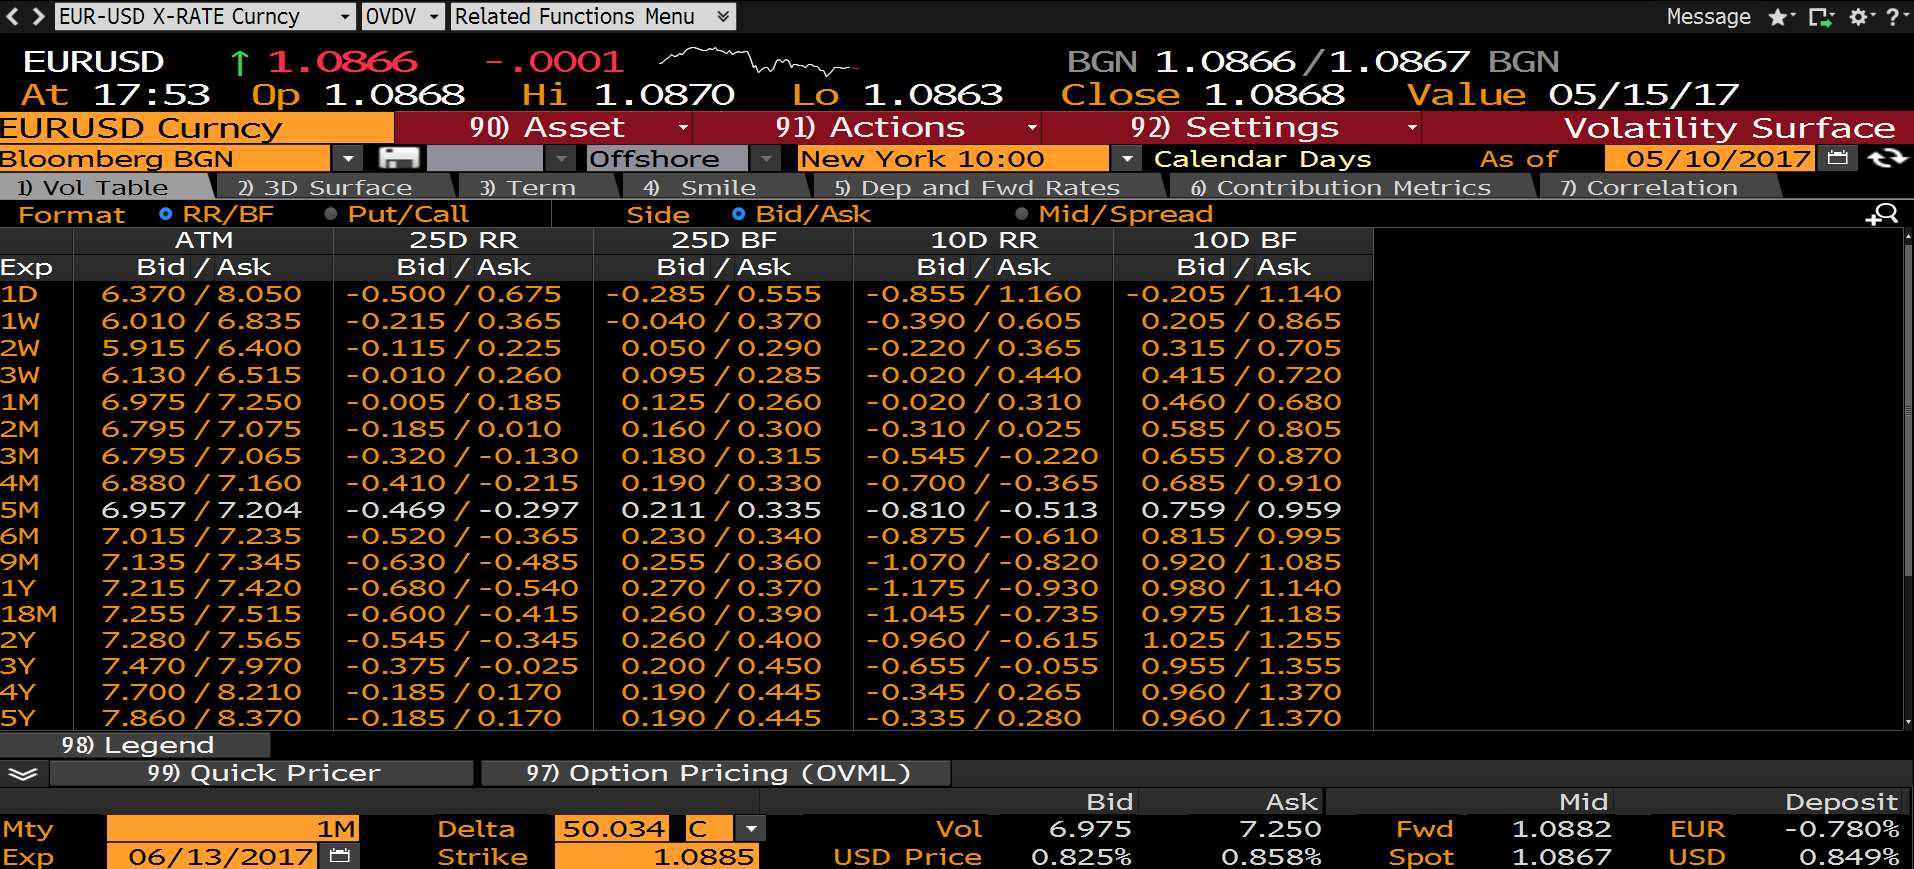
\includegraphics[scale=0.3]{./Testing-data/VolMatrix/EURUSD_1M_vol.png} 
	\caption{Volatility matrix data in the bid/ask format in terms of ATM, $10\Delta$, and $25\Delta$ butterflies (BF) and risk reversals (RR), observed on May 10, 2017. Source: \textit{Bloomberg}}
	\label{fig:label} % insert suitable label, this is used to refer to a fig from within the text as shown above
\end{figure}
\noindent
In order to verify the price calculated by using Vanna-Volga model, two benchmark sources (Bloomberg pricing model and \textit{investing.com} with price provided by \textit{Sentry Derivatives}) for FX derivatives had been put in \textit{Appendix A.3}. Since Vanna-Volga is an analytically derived correction to Black-Scholes model, the price calucluated by Black-Scholes model also had been included for analysis.
\newline
\newline
The interest rates used for Vanna-Volga model and Black-Scholes model was obtained from \textit{www.tradingeconomics.com} and listed in the following table.

\begin{table}[htb]
\centering
\caption{{FX interest rates observed on May 10, 2017}}
\begin{tabular}{ccc}
\hline	\hline % insert double horizontal line
Symbol & USD & EUR   \\ [1ex]% heading
\hline
Rates & 1.00\% & 0.00\%    \\ [1ex]
\hline
\end{tabular}
\label{table:FX_rates}
\end{table}

\subsection{Model Implementation}
As the volatility matrix obtianed from Bloomberg is in the bid/ask format, the averaged mid volatility was used for Black-Scholes model and Vanna-Volga model. The mid volatility matrix data of three FX derivatives were list below. And we consider that live exchange rate as the initial price of FX options $S_0$.
\newline
\newline
Since Vanna-Volga model is limited to the short-dated (tipically less than 1Y) FX options, a test of EUR/USD call options with 1Y maturity also had been conducted with same procedure of 1M maturity.
\begin{table}[htb]
\centering
\caption{Mid volatility matrix of EUR/USD with 1M maturity}
\begin{tabular}{ccccccc}
\hline \hline
FX derivatives & ATM  & 25D RR  & 25D BF  & 10D RR  & 10D BF & $S_0$\\ [0.5ex]
\hline 
EUR/USD  & 7.1125 &0.09& 0.1925 &0.145 &0.57&1.0866 \\[0.5ex]
\hline
\end{tabular}
\end{table}

\begin{table}[htb]
	\centering
	\caption{Mid volatility matrix of EUR/USD with 1Y maturity}
	\begin{tabular}{ccccccc}
		\hline \hline
		FX derivatives & ATM  & 25D RR  & 25D BF  & 10D RR  & 10D BF & $S_0$\\ [0.5ex]
		\hline 
		EUR/USD  & 7.415&	-0.685&	0.325&	-1.175	&1.065 &1.0923\\[0.5ex]
		\hline
	\end{tabular}
\end{table}

\noindent
With the conventions and definitions specified in \textbf{Technical Specification}, the implementation of Black-Scholes model and Vanna-Volga model of FX derivatives had been coded in jupyter notebook with Python 3.5 in \textit{Appendix A.3}.

\section{Testing Results}
In order to compare the prices calculated from Vanna-Volga to the benchmark prices easily, we define the price to be \% FOR (foreign currency). For example, we use \% EUR to be the price form of Vanna-Volga model for EUR/USD options.
\subsection{Short-dated Maturity}
The results from the implemented codes with EUR/USD call option had been put in the table. The details of the prices of four methods corresponding to the strike could be found in \textit{Appendix A.3}.

\begin{table}[htb]
\centering
\caption{Prices of EUR/USD call option with 1M matiruty}
\begin{tabular}{ccccc}
\hline \hline
Strike & Heston & investing.com & BS & Vanna-Volga \\ [0.5ex]
\hline
1.065 &	0.023241&	0.0233	&0.024682&	0.023363 \\ 
1.070&	0.019381&	0.0195&	0.020663&	0.019671\\
1.075	&0.015802&	0.0160&	0.016970&	0.016277 \\
1.080	&0.012571&	0.0128&	0.013649&	0.013224\\
1.085	&0.009770&	0.0101&	0.010733&	0.010544 \\ [0.5ex]
\hline
\end{tabular}
\label{table:prices-1M}
\end{table}

\noindent
From the table, we could find that the prices of Vanna-Volga were close to the prices of Bloomberg and investing.com. In particular, Vanna-Volga prices were very close to the prices used in investing.com. In order to visulize the results, a figure contained all the prices had been put in the below.

\begin{figure}[htb]
	\centering
\includegraphics[scale=0.4]{./Testing-data/Python-codes/Python-4prices-1M.png} 
\caption{Prices of EUR/USD call options with 1M maturity. Data observed on May 10, 2017}
\label{fig:prices-label} % insert suitable label, this is used to refer to a fig from within the text as shown above
\end{figure}

\noindent
The figure clearly showed that the prices calculated through Vanna-Volga model were very close to the benchmark prices. Besides, as we might see, the Black-Scholes prices (green line) were far away from the benchmark prices compared to Vanna-Volga prices. This figure was consistent with the purpose of the Vanna-Volga model, which is that Vanna-Volga model is an analytically derived correction by capturing the greeks of vanna and volga to Black-Scholes model.

\subsection{1Y Maturity}

Following the same procedure, we got the result as following.

\begin{table}[htb]
	\centering
	\caption{Prices of EUR/USD call option with 1Y matiruty}
	\begin{tabular}{ccccc}
		\hline \hline
		Strike & Heston & investing.com & BS & Vanna-Volga \\ [0.5ex]
		\hline
		1.05 &	0.069127&	0.0695&	0.065060&	0.058870 \\ 
		1.06&	0.062125&	0.0623	&0.058001&	0.052372\\
		1.07&	0.055455&	0.0555&	0.051381&	0.046276 \\
		1.08&	0.049155&	0.0490	&0.045220&	0.040596\\
		1.09&	0.043257&	0.0429	&0.039532&	0.035339 \\ [0.5ex]
		\hline
	\end{tabular}
	\label{table:prices-1Y}
\end{table}
\noindent
From the table, we found that two benchmark prices (Heston from Bloomberg pricing tools and prices from \textit{investing.com}) are very close. However, Black-Scholes prices were much far away from the benchmark prices and the Vanna-Volga prices were even far away from the benchmark prices. In order to visulize the results, a figure contained all the prices had been put in the below.

\begin{figure}[htb]
	\centering
	\includegraphics[scale=0.4]{./Testing-data/Python-codes/Python-4prices-1Y.png} 
	\caption{Prices of EUR/USD call options with 1Y maturity. Data observed on May 12, 2017}
	\label{fig:prices-1Y-MAY12} % insert suitable label, this is used to refer to a fig from within the text as shown above
\end{figure}
\noindent
The figure clearly showed that both Black-Scholes prices and Vanna-Volga prices were far away from the benchmark prices, which implied that the Black-Scholes model and Vanna-Volga model were not good for long-dated maturity FX options.

\subsection{Test Conclusion}
\noindent
\textbf{Therefore, we conclued that the model is valid and appropriate for short-dated (less than 1Y) maturity FX vanilla options pricing.} As the limitation of the report, only FX vanilla options pricing had been tested. However, Agnieszka Janek showed that Vanna-Volga model was also good for pricing first-generation FX options, e.g., FX barrier options. His paper had been included in the references list.


\chapter{Model Strengths and Weaknesses}


\section{Strengths}

\paragraph{}

As we all known that Black-Scholes model is most often used to price vanilla options. However, the parameters used in Black-Scholes model are far from market quotations. The main reason is the unrealistic assumption that the volatility remain constant throught the lifetime of the vanilla options. Besides, the volatility surfaces of FX derivatives tend to be smile shaped or skewed. Thus, Black-Scholes model is insufficient in FX market.
	
\paragraph{}

There are models, such as Heston model and local volatility model, could capture and well replicate the smile shaped or skewed volatility surface of FX derivatives. However, none of them is easy to implement and require delicate calibration. Therefore, compare to other models used for FX derivatives, Vanna-Volga model has following strengths:

\begin{itemize}
	\item Vanna-Volga is easy to implement, comparing to other models
	\item Vanna-Volga is simple and no or few calibration is needed
	\item Vanna-Volga is very efficient in computation, i.e., the calculation speed is significantly better than Heston model or local volatility model
	\item The instruments used for constructing the Vanna-volga model are very liquid in FX market. Typically, people are using straddle, risk reversal, and butterfly to construct Vanna-Volga framework
	\item Vanna-Volga is an analytically derived correction by capturing the greeks of vanna and volga to Black-Scholes model, i.e., by using vega, vanna and volga of the options. Therefore, it is easy to understand intiuitively.
\end{itemize}


\section{Weaknesses}
\paragraph{}
Even though Vanna-Volga model also known as \textit{trader's rule of thmb} and has some features listed above, it dose have some drawbacks or conditions need to be understood before using it. Typical weaknesses of Vanna-Volga model are following:

\begin{itemize}
	\item Vanna-Volga is precise when the maturity of options is up to 1 year, since the model assumes constant interest rates which does not lead to significantly mispricing for short maturity options in FX market.
	\item The application of Vanna-Volga model is limited to plain vanilla options and first-generation exotic options, such as barrier options, since it cannot fully replicate the volatility surface. However, many of the options in FX market is vanilla or first-generation exotic options.
	\item Vanna-Volga model perform well when the volatility surface is standard (such as smile shaped, typical skewed) of FX derivatives.
\end{itemize}



\appendix
\chapter{}
\section{Data Sources}

The prices of EUR/USD in \textit{www.investing.com} is following:
\begin{figure}[htb]
	\centering
	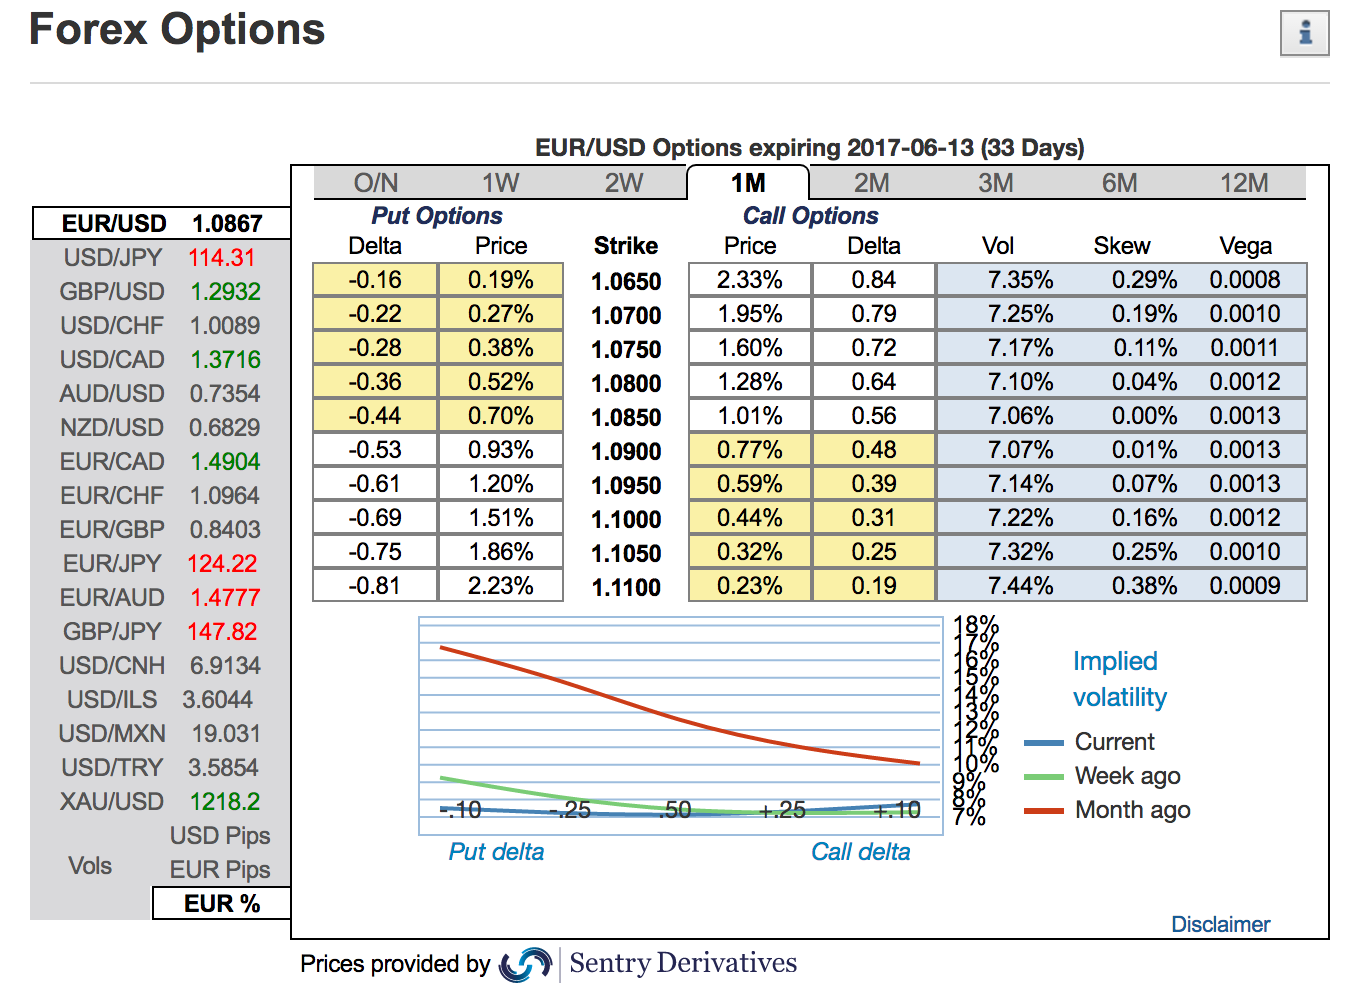
\includegraphics[scale=0.4]{./Testing-data/EURUSD_1M_investing.png} 
	\caption{EUR/USD call prices from investing.com}
	\label{fig:prices-investing.com} % insert suitable label, this is used to refer to a fig from within the text as shown above
\end{figure}

Since Bloomber has its own pricing model for FX options, the prices of EUR/USD call options with different strikes are obtained in Bloomberg terminal and listed below (using strike 1.065 as example).

\begin{figure}[htb]
	\centering
	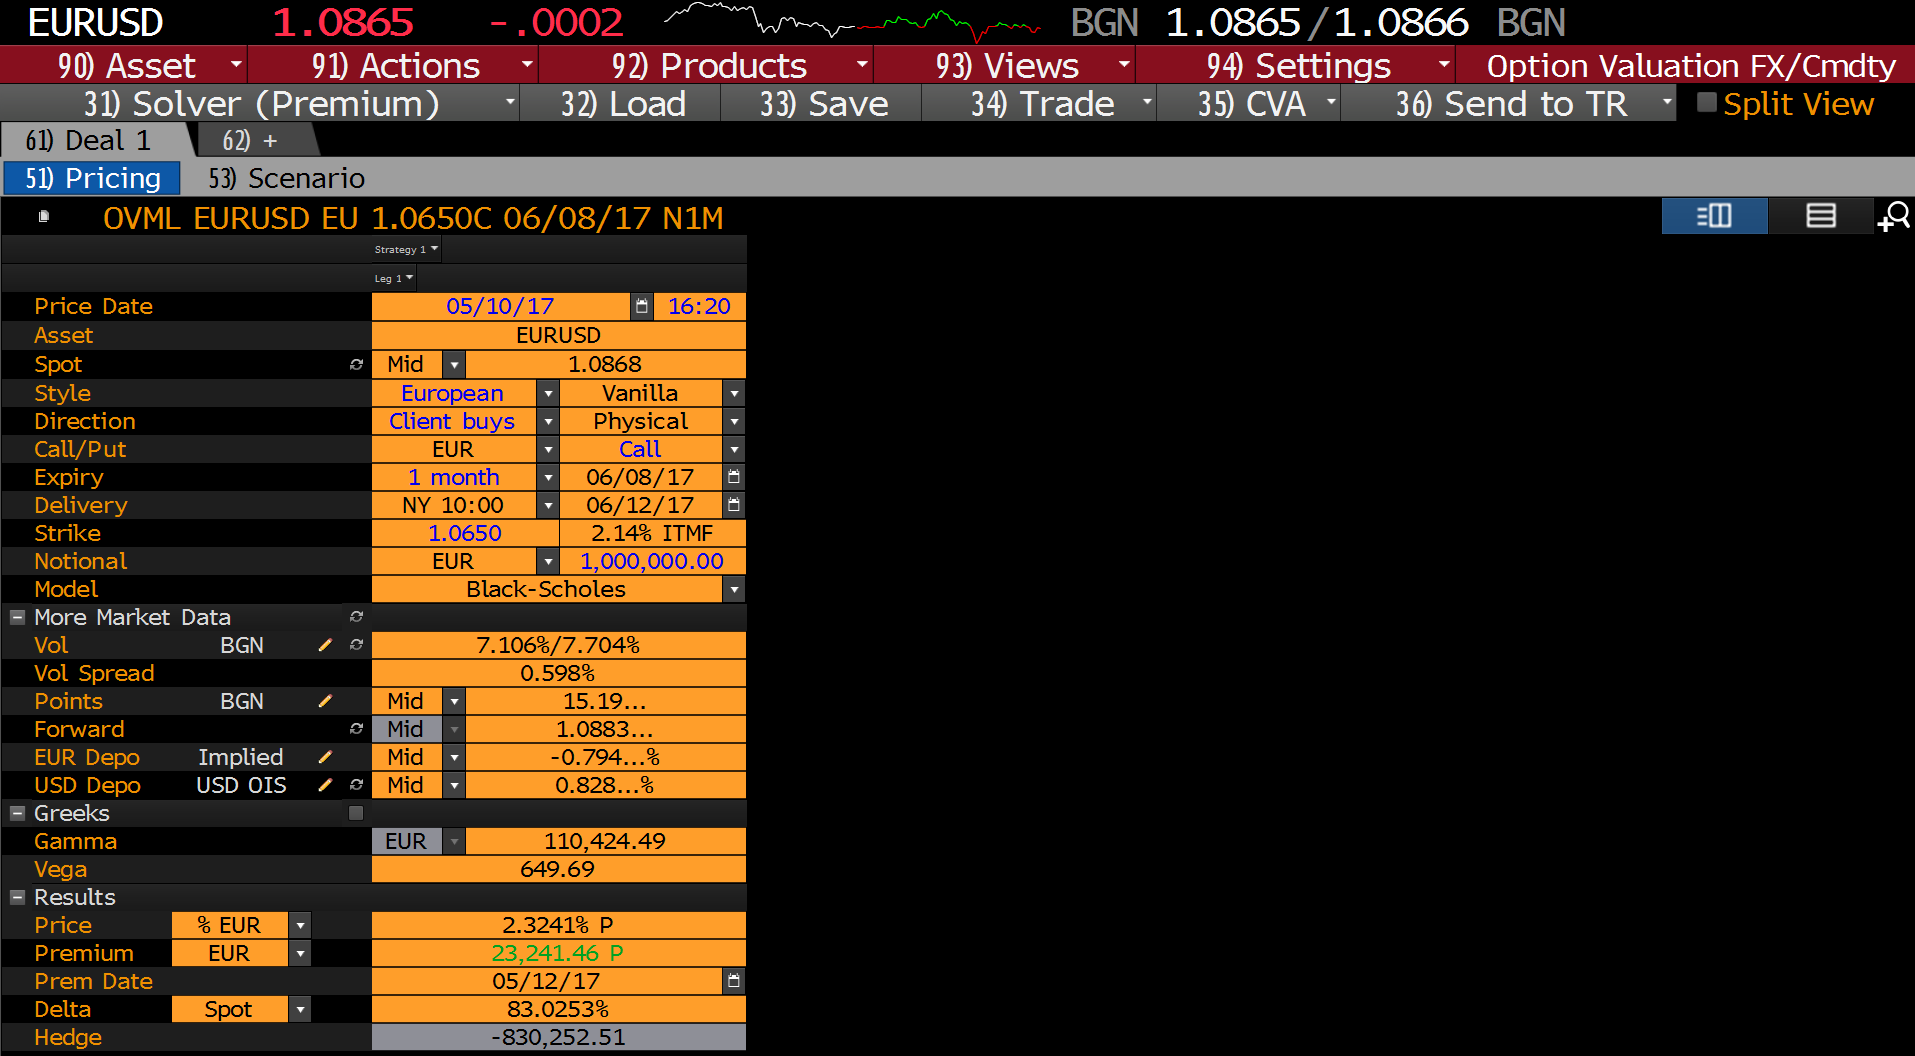
\includegraphics[scale=0.3]{./Testing-data/Price-Bloomberg/EURUSD1065.PNG} 
	\caption{EUR/USD call prices with strike 1.065}
	
	\label{fig:prices-investing.com} % insert suitable label, this is used to refer to a fig from within the text as shown above
\end{figure}


\newpage
\section{Definitions}
25 and 10 $\Delta$-Risk-reversal (RR) volatility:
\begin{align}
\sigma_{RR25}&=\sigma_{25\Delta C}-\sigma_{25\Delta P}\\
\sigma_{RR10}&=\sigma_{10\Delta C}-\sigma_{10\Delta P}
\end{align}
\newline
25 and 10 $\Delta$-Butterfly (BF) volatility:
\begin{align}
\sigma_{BF25}=\frac{1}{2}\left[\sigma_{25\Delta C}+\sigma_{25\Delta P}\right]-\sigma_{ATM}\\
\sigma_{BF10}=\frac{1}{2}\left[\sigma_{10\Delta C}+\sigma_{10\Delta P}\right]-\sigma_{ATM}
\end{align}
\newline
These yields to the following equations:
\begin{align}
\sigma_{25\Delta C}=\sigma_{ATM}+\sigma_{BF25}+\frac{1}{2}\sigma_{RR25}\\
\sigma_{25\Delta P}=\sigma_{ATM}+\sigma_{BF25}-\frac{1}{2}\sigma_{RR25}\\
\sigma_{10\Delta C}=\sigma_{ATM}+\sigma_{BF10}+\frac{1}{2}\sigma_{RR10}\\
\sigma_{10\Delta P}=\sigma_{ATM}+\sigma_{BF10}-\frac{1}{2}\sigma_{RR10}
\end{align}
\newline
Strike retrived from deltas can be calculated through following equation:
\begin{align}
K=S_0e^{(r_d-r_f)T-\phi \sigma \sqrt{T} N^{-1}(\phi \Delta)+\frac{1}{2}\sigma^2T}
\end{align}
where $\phi=1$ for call, and $\phi=-1$ for put.

\section{Python Code of Vanna-Volga Model}
The codes of Vanna-Volga model had been implemented in jupyter notebook with kernel Python 3.5. Details of the codes could be found in the corresponding jupyter notebook with name as "MTH9845\_final\_project\_codes.ipynb". The jupyter notebook also had been converted to a pdf file with name as "MTH9845\_final\_project\_codes.pdf". Please see the details in the seperate files

\cleardoublepage
%\pagebreak
\phantomsection
\addcontentsline{toc}{chapter}{References}
\begin{thebibliography}{99}

\bibitem{citation-1-name-here}<Name of the reference here>,\ \url{<url here>}

\bibitem{citation-2-name-here}<Name of the reference here>,\ \url{<url here>}

\end{thebibliography}


\end{document}
